\section{Week 4: Counting and Probability I}
\subsection*{Reading}
Epp \S 9.1--9.4.

\subsection*{Learning objectives}
\begin{itemize}
  \item Build sample spaces and events for basic probability models.
  \item Apply the multiplication rule to count outcomes.
  \item Apply the addition rule and inclusion--exclusion for two sets.
  \item Use the pigeonhole principle to force collisions.
  \item Count permutations and arrangements with restrictions.
\end{itemize}

\subsection*{Key definitions and facts}

\begin{definition}[Sample space and event]
A \textbf{sample space} $S$ is the set of all possible outcomes of an experiment. An \textbf{event} is a subset $E \subseteq S$. The event $E$ \textbf{occurs} if the outcome of the experiment is in $E$.
\end{definition}

\begin{definition}[Probability (equally likely outcomes)]
If all outcomes in a finite sample space $S$ are equally likely, then for any event $E$:
\[
P(E) = \frac{|E|}{|S|}
\]
\end{definition}

\begin{theorem}[Basic probability properties]
For any events $A, B$ in sample space $S$:
\begin{enumerate}
  \item $0 \leq P(A) \leq 1$
  \item $P(S) = 1$ and $P(\emptyset) = 0$
  \item $P(A^c) = 1 - P(A)$ where $A^c = S \setminus A$ is the complement of $A$
  \item If $A \cap B = \emptyset$, then $P(A \cup B) = P(A) + P(B)$
\end{enumerate}
\end{theorem}

\begin{theorem}[Multiplication rule (product rule)]
If a procedure can be broken into $k$ successive steps, where step 1 can be done in $n_1$ ways, step 2 can be done in $n_2$ ways (regardless of step 1's outcome), \ldots, step $k$ can be done in $n_k$ ways, then the total number of ways to complete the procedure is:
\[
n_1 \times n_2 \times \cdots \times n_k
\]
\end{theorem}

\begin{theorem}[Addition rule (sum rule)]
If a task can be done either by method $A$ (in $n_1$ ways) or by method $B$ (in $n_2$ ways), and the two methods are mutually exclusive (no overlap), then the total number of ways is:
\[
n_1 + n_2
\]
\end{theorem}

\begin{theorem}[Inclusion-exclusion (two sets)]
For any finite sets $A$ and $B$:
\[
|A \cup B| = |A| + |B| - |A \cap B|
\]
For probabilities:
\[
P(A \cup B) = P(A) + P(B) - P(A \cap B)
\]
\end{theorem}

\begin{theorem}[Inclusion-exclusion (three sets)]
For finite sets $A$, $B$, $C$:
\[
|A \cup B \cup C| = |A| + |B| + |C| - |A \cap B| - |A \cap C| - |B \cap C| + |A \cap B \cap C|
\]
\end{theorem}

\begin{definition}[Permutation]
A \textbf{permutation} of a set is an arrangement of its elements in a sequence. The number of permutations of $n$ distinct objects is:
\[
n! = n \times (n-1) \times (n-2) \times \cdots \times 2 \times 1
\]
By convention, $0! = 1$.
\end{definition}

\begin{definition}[$r$-permutation]
An \textbf{$r$-permutation} of $n$ objects is an ordered arrangement of $r$ objects chosen from $n$ distinct objects. The count is:
\[
P(n, r) = \frac{n!}{(n-r)!} = n \times (n-1) \times \cdots \times (n-r+1)
\]
\end{definition}

\begin{theorem}[Pigeonhole principle (basic)]
If $n + 1$ objects are placed into $n$ boxes, then at least one box contains at least 2 objects.
\end{theorem}

\begin{theorem}[Pigeonhole principle (generalized)]
If $n$ objects are placed into $k$ boxes, then at least one box contains at least $\lceil n/k \rceil$ objects.
\end{theorem}

\begin{keyresult}
The pigeonhole principle guarantees existence but doesn't tell you \emph{which} box has multiple objects. It's powerful for proving that certain configurations must exist.
\end{keyresult}

\begin{definition}[Distinguishable vs. indistinguishable]
Objects are \textbf{distinguishable} if we can tell them apart; \textbf{indistinguishable} if we cannot. Similarly for boxes/positions.
\begin{itemize}
  \item Distinguishable objects into distinguishable boxes: use multiplication rule
  \item Indistinguishable objects into distinguishable boxes: use combinations (Week 5)
\end{itemize}
\end{definition}

\subsection*{Counting techniques}

\begin{strategy}
\textbf{Direct counting:} Count the desired outcomes directly using multiplication/addition rules.

\textbf{Complement counting:} Sometimes it's easier to count what you \emph{don't} want:
\[
|\text{desired}| = |\text{total}| - |\text{undesired}|
\]
\end{strategy}

\begin{definition}[Possibility tree]
A \textbf{possibility tree} (or decision tree) is a diagram that systematically lists all possible outcomes of a multi-step process. Each branch point represents a choice, and each path from root to leaf represents one complete outcome. The total count equals the number of leaves.
\end{definition}

\begin{example}[Possibility tree]
How many 2-letter strings over $\{A, B, C\}$ have no repeated letters?

\emph{Solution via possibility tree:}
\begin{center}
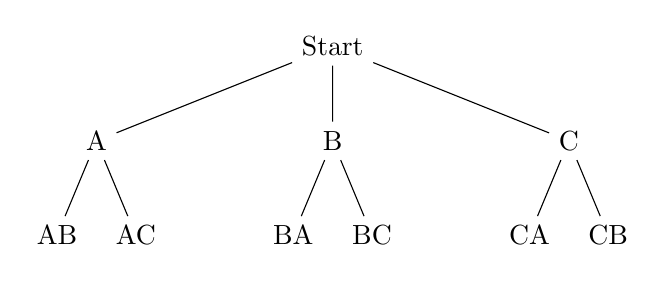
\begin{tikzpicture}[level distance=1.2cm, sibling distance=2cm,
  level 1/.style={sibling distance=3cm},
  level 2/.style={sibling distance=1cm}]
\node {Start}
  child {node {A}
    child {node {AB}}
    child {node {AC}}
  }
  child {node {B}
    child {node {BA}}
    child {node {BC}}
  }
  child {node {C}
    child {node {CA}}
    child {node {CB}}
  };
\end{tikzpicture}
\end{center}
First letter: 3 choices. Second letter: 2 choices (can't repeat). Total: $3 \times 2 = 6$ strings.
\end{example}

\begin{keyresult}
Possibility trees are most useful when:
\begin{itemize}
  \item The number of outcomes is small enough to draw
  \item Choices at each step depend on previous choices
  \item You need to verify your counting is correct
\end{itemize}
For larger problems, use the multiplication/addition rules directly.
\end{keyresult}

\begin{definition}[With vs. without replacement]
\begin{itemize}
  \item \textbf{With replacement:} After selecting an object, it goes back into the pool. Selections are independent.
  \item \textbf{Without replacement:} Once selected, an object is removed from the pool. Later selections have fewer choices.
\end{itemize}
\end{definition}

\begin{proposition}[Counting sequences]
From a set of $n$ distinct elements:
\begin{itemize}
  \item Sequences of length $k$ \textbf{with replacement}: $n^k$
  \item Sequences of length $k$ \textbf{without replacement}: $P(n,k) = \frac{n!}{(n-k)!}$
\end{itemize}
\end{proposition}

\subsection*{Worked examples}

\begin{example}
A license plate consists of 3 letters followed by 3 digits. How many license plates are possible?

\emph{Solution.} Using the multiplication rule:
\begin{itemize}
  \item 3 letters: $26 \times 26 \times 26 = 26^3$ choices (with replacement)
  \item 3 digits: $10 \times 10 \times 10 = 10^3$ choices
\end{itemize}
Total: $26^3 \times 10^3 = 17,576 \times 1000 = 17,576,000$.
\end{example}

\begin{example}
How many 3-letter strings over $\{A, B, C, D\}$ have no repeated letters?

\emph{Solution.} This is a 3-permutation of 4 objects:
\[
P(4, 3) = 4 \times 3 \times 2 = 24
\]
Alternatively: First letter: 4 choices. Second letter: 3 choices (can't repeat first). Third letter: 2 choices.
\end{example}

\begin{example}
A fair die is rolled twice. What is the probability that the sum is 7?

\emph{Solution.}
\begin{itemize}
  \item Sample space: All pairs $(a, b)$ with $a, b \in \{1, 2, 3, 4, 5, 6\}$. Size: $6 \times 6 = 36$.
  \item Event $E$: pairs summing to 7. These are $(1,6), (2,5), (3,4), (4,3), (5,2), (6,1)$. Size: 6.
\end{itemize}
\[
P(E) = \frac{6}{36} = \frac{1}{6}
\]
\end{example}

\begin{example}
How many 5-bit binary strings contain at least one 1?

\emph{Solution (complement counting).}
\begin{itemize}
  \item Total 5-bit strings: $2^5 = 32$
  \item Strings with no 1s: just $00000$, so 1
\end{itemize}
Strings with at least one 1: $32 - 1 = 31$.
\end{example}

\begin{example}
How many integers in $\{1, 2, \ldots, 100\}$ are divisible by 2 or 3?

\emph{Solution (inclusion-exclusion).}
Let $A = \{n : 2 \mid n\}$ and $B = \{n : 3 \mid n\}$.
\begin{itemize}
  \item $|A| = \lfloor 100/2 \rfloor = 50$
  \item $|B| = \lfloor 100/3 \rfloor = 33$
  \item $|A \cap B| = |\{n : 6 \mid n\}| = \lfloor 100/6 \rfloor = 16$
\end{itemize}
\[
|A \cup B| = 50 + 33 - 16 = 67
\]
\end{example}

\begin{example}
Prove: Among any 13 people, at least two share a birth month.

\emph{Solution.} There are 12 months (boxes) and 13 people (objects). By the pigeonhole principle, at least one month contains at least 2 people.
\end{example}

\begin{example}
Prove: In any set of 6 integers, there exist two with the same remainder when divided by 5.

\emph{Solution.} Remainders modulo 5 are in $\{0, 1, 2, 3, 4\}$ (5 boxes). With 6 integers (objects), by pigeonhole, at least two have the same remainder.
\end{example}

\begin{example}
How many ways can 8 people sit in a row if two specific people (Alice and Bob) must sit together?

\emph{Solution.} Treat Alice and Bob as a single ``super-person.'' Then we arrange 7 objects in a row: $7!$ ways. But Alice and Bob can be in either order within their block: 2 ways.

Total: $7! \times 2 = 5040 \times 2 = 10080$.
\end{example}

\begin{example}
How many ways can 8 people sit in a row if Alice and Bob must NOT sit together?

\emph{Solution (complement counting).}
\begin{itemize}
  \item Total arrangements: $8! = 40320$
  \item Arrangements where they sit together: $10080$ (from previous example)
\end{itemize}
Answer: $40320 - 10080 = 30240$.
\end{example}

\begin{example}
A committee of 5 is to be chosen from 8 candidates. In how many ways can this be done if the order of selection matters?

\emph{Solution.} This is a 5-permutation of 8:
\[
P(8, 5) = 8 \times 7 \times 6 \times 5 \times 4 = 6720
\]
\end{example}

\begin{example}
Prove: Among any 5 points placed inside a unit square, at least two are within distance $\frac{\sqrt{2}}{2}$ of each other.

\emph{Solution.} Divide the unit square into 4 smaller squares of side $\frac{1}{2}$. By pigeonhole, at least two of the 5 points lie in the same small square. The maximum distance between two points in a square of side $\frac{1}{2}$ is the diagonal length: $\frac{\sqrt{2}}{2}$.
\end{example}

\begin{commonmistake}
\textbf{Overcounting.} When counting arrangements, make sure you're not counting the same configuration multiple times. Ask yourself:
\begin{itemize}
  \item Does order matter? (permutation vs. combination)
  \item Are objects distinguishable?
  \item Are positions/boxes distinguishable?
\end{itemize}
\end{commonmistake}

\begin{commonmistake}
\textbf{Misapplying the multiplication rule.} The multiplication rule requires that the number of choices at each step is \emph{independent} of previous choices (or carefully accounted for). If earlier choices affect later options, you must account for this.
\end{commonmistake}

\begin{goingdeeper}[Going Deeper: The Algebra of Types]
The counting rules we've learned---multiplication and addition---have a surprising connection to types in programming. This connection reveals why these rules are so fundamental.

\subsubsection*{Types Have Sizes}

In programming, a \emph{type} is a set of values. We can count how many values a type has:
\begin{center}
\begin{tabular}{lcc}
\textbf{Type} & \textbf{Description} & \textbf{Size} \\
\hline
\texttt{Void} & empty type (no values) & 0 \\
\texttt{Unit} or \texttt{()} & type with one value & 1 \\
\texttt{Bool} & \texttt{True} or \texttt{False} & 2 \\
\texttt{Char} & ASCII characters & 128 (or 256)
\end{tabular}
\end{center}

\subsubsection*{Products and Sums of Types}

Now here's the magic. If we combine types:
\begin{itemize}
  \item \textbf{Product type} $(A, B)$ (pairs): $|A \times B| = |A| \times |B|$
  \item \textbf{Sum type} \texttt{Either A B}: $|A + B| = |A| + |B|$
\end{itemize}

This is exactly the multiplication and addition rules for counting!

\textbf{Example.} The type \texttt{(Bool, Bool)} has $2 \times 2 = 4$ values:
\[
\texttt{(True, True), (True, False), (False, True), (False, False)}
\]

\textbf{Example.} The type \texttt{Either Bool ()} has $2 + 1 = 3$ values:
\[
\texttt{Left True, Left False, Right ()}
\]

\subsubsection*{Why the Names ``Product'' and ``Sum''?}

This isn't a coincidence! The names come from the fact that type sizes multiply and add. The categorical perspective (from Week 2) explains why:
\begin{itemize}
  \item Products satisfy the universal property of products
  \item Sums (coproducts) satisfy the dual universal property
\end{itemize}

\subsubsection*{Algebraic Laws}

These type operations satisfy the same laws as arithmetic:
\begin{itemize}
  \item $A \times 1 \cong A$ (pairing with unit adds no information)
  \item $A + 0 \cong A$ (sum with empty type is just $A$)
  \item $A \times (B + C) \cong (A \times B) + (A \times C)$ (distributivity)
  \item $A \times B \cong B \times A$ (commutativity)
\end{itemize}

\subsubsection*{Exercises: Types and Counting}

\begin{enumerate}
  \item How many values does the type \texttt{(Bool, Bool, Bool)} have? List them.

  \item How many values does \texttt{Either Bool Bool} have? How is this different from \texttt{(Bool, Bool)}?

  \item If type $A$ has 3 values and type $B$ has 4 values, how many values does $A \times B$ have? How many does $A + B$ have?

  \item The type \texttt{Maybe A} is defined as \texttt{Either () A} (either ``nothing'' or a value of type $A$). If $|A| = n$, what is $|\texttt{Maybe } A|$?

  \item Verify the distributive law by counting: if $|A| = 2$, $|B| = 3$, $|C| = 1$, check that $|A \times (B + C)| = |A \times B| + |A \times C|$.

  \item \textbf{Challenge:} Function types $A \to B$ have $|B|^{|A|}$ values (every function is a choice of output for each input). Verify this for $A = \texttt{Bool}$ and $B = \{1, 2, 3\}$ by listing all functions.
\end{enumerate}
\end{goingdeeper}

\subsection*{Practice}
\begin{enumerate}
  \item A fair die is rolled twice. What is the probability the sum is 7?

  \item How many 5-bit binary strings contain at least one 1?

  \item Use inclusion--exclusion to count integers in $\{1, \ldots, 100\}$ divisible by 2 or 3.

  \item Use the pigeonhole principle to show that among 13 people, two share a birth month.

  \item How many 4-digit PINs (using digits 0--9) have no repeated digits?

  \item A standard deck has 52 cards. How many 5-card hands are possible? (Order doesn't matter---use $\binom{52}{5}$ from Week 5, or just set up the problem.)

  \item How many ways can 6 different books be arranged on a shelf if two specific books must be at the ends?

  \item How many bit strings of length 8 start with 1 or end with 00?

  \item Prove: Among any 10 integers, there exist two whose difference is divisible by 9.

  \item A restaurant offers 3 appetizers, 5 main courses, and 2 desserts. How many different 3-course meals are possible?

  \item How many permutations of ABCDEF contain ABC as a consecutive substring?

  \item Prove: If 5 points are selected from the integer lattice points in $\{0,1,2\}^2$, then two of them have midpoint that is also a lattice point.
\end{enumerate}
